% sections/03_classification.tex
\section{Classification}
\label{sec:classification}

Classification is the task of assigning each observation to one of a fixed set of categories. In this study the categories are the three penguin species, and the predictors are physical traits of the individual. Two models are compared, logistic regression and a decision tree. Each model is trained under two feature configurations: one using only the four continuous physical traits, and one adding the sex of the individual. Both configurations are trained on two disjoint training subsets that share the same test set, so that the effect of sex can be separated from the effect of the specific training rows. The design of those subsets is covered in Section~\ref{sec:robustness}; this section focuses on the models themselves and on the marginal contribution of sex.

The target variable is \texttt{species}. The features are bill length, bill depth, flipper length and body mass, and in the second configuration also sex. Both models are built with \texttt{scikit-learn}, use \texttt{random\_state=42} for reproducibility, are trained with the \texttt{fit} method, and produce predictions with the \texttt{predict} method.

\subsection{Logistic Regression}

Logistic regression is a linear model for classification. For each class it computes a linear combination of the predictors and passes the result through the logistic function, which produces a probability between 0 and 1. The predicted class is the one with the highest probability. Because the model is linear, its decision boundaries are hyperplanes in the feature space, an assumption that is restrictive in general but works well when the classes are well separated. The \texttt{scikit-learn} implementation applies L2 regularization by default, which helps control overfitting when the number of features is small.

\begin{figure}[htbp]
	\centering
	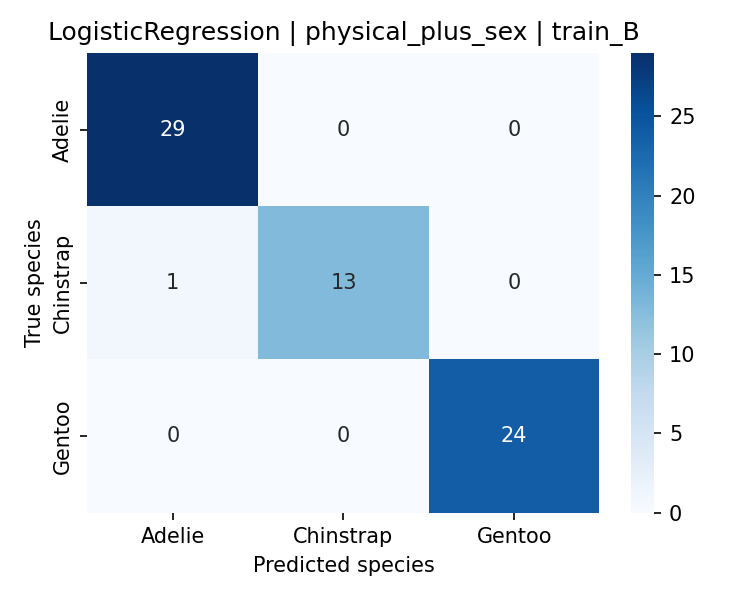
\includegraphics[width=0.7\textwidth]{figures/cm_LogisticRegression_physical_plus_sex_train_B.png}
	\caption{Confusion matrix for logistic regression with sex as a predictor, trained on subset B of the training data.}
	\label{fig:cm_logreg}
\end{figure}

On the shared test set, logistic regression with sex as a predictor reaches an accuracy of 0.985 and a weighted precision of 0.986 when trained on subset B, which is 66 correct predictions out of 67. The confusion matrix shows a single error: one Chinstrap individual is predicted as Adelie. Adelie and Gentoo are classified perfectly. The Chinstrap-Adelie confusion is consistent with the data alone, as the two species overlap in bill dimensions and are only separated cleanly by combining several traits.

\subsection{Decision Tree}

A decision tree partitions the feature space recursively. At each node it selects the feature and threshold that split the training data with the lowest impurity, measured by the Gini index. The process continues until the leaves are pure or a stopping criterion is met. Trees make no assumption about the shape of the decision boundary, so they can capture non-linear relations and interactions between predictors. The trade-off is that an unconstrained tree grows until it memorizes the training set, which is why hyperparameter tuning is needed. That step is covered in Section~\ref{sec:hyperparameter_tuning}.

\begin{figure}[htbp]
	\centering
	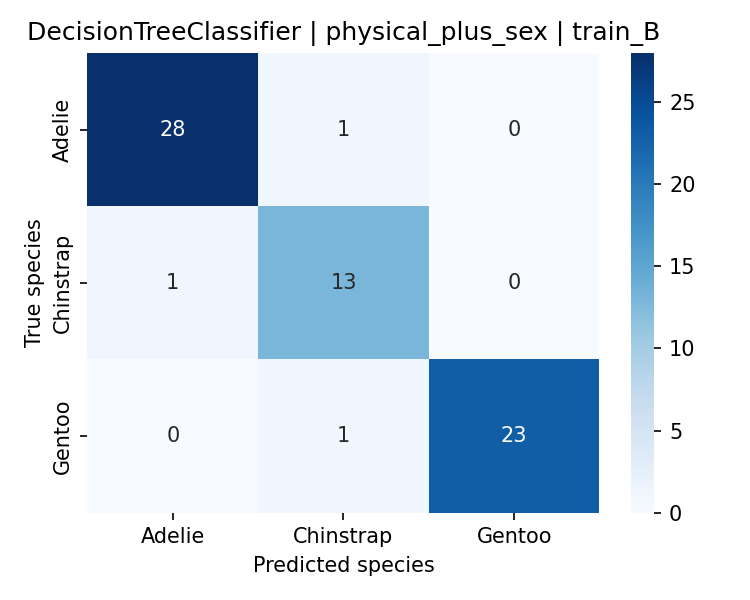
\includegraphics[width=0.7\textwidth]{figures/cm_DecisionTreeClassifier_physical_plus_sex_train_B.png}
	\caption{Confusion matrix for the decision tree with sex as a predictor, trained on subset B of the training data.}
	\label{fig:cm_tree}
\end{figure}

On the same test set, the decision tree with sex reaches an accuracy of 0.955 and a weighted precision of 0.955 when trained on subset B, which is 64 correct predictions out of 67. The confusion matrix shows three errors: one Adelie predicted as Chinstrap, one Chinstrap predicted as Adelie, and one Gentoo predicted as Chinstrap. The first two are consistent with the morphological overlap between Adelie and Chinstrap. The third is more surprising, since Gentoo is well separated from the other two species, and it reflects the tendency of an unconstrained tree to split the training data very finely and then generalize unevenly on a small test set.

\subsection{Effect of Sex on Classification}

Because each model is trained on two disjoint training subsets, the metrics vary slightly between runs. Table~\ref{tab:cls_metrics} reports the range of accuracy and weighted precision across the two subsets for each configuration.

\begin{table}[htbp]
	\centering
	\caption{Classification metrics on the shared test set. Ranges indicate the variation across the two disjoint training subsets.}
	\label{tab:cls_metrics}
	\begin{tabular}{lll}
		\toprule
		Model & Accuracy & Weighted precision \\
		\midrule
		Logistic regression (without sex) & 0.925 & 0.936 \\
		Logistic regression (with sex)    & 0.970 to 0.985 & 0.972 to 0.986 \\
		Decision tree (without sex)       & 0.910 to 0.955 & 0.914 to 0.957 \\
		Decision tree (with sex)          & 0.910 to 0.955 & 0.914 to 0.957 \\
		\bottomrule
	\end{tabular}
\end{table}

For logistic regression, adding sex raises accuracy by 0.045 on subset A and by 0.060 on subset B, which is the same as moving from 0.925 to 0.970 and from 0.925 to 0.985 respectively. The direction of the change is the same in both runs. For the decision tree, the metrics are indistinguishable on this test set with and without sex. This suggests that the splits selected by the tree already encode the information that sex provides, which is plausible given that male and female penguins differ mainly in body size, a variable the tree can split on directly.

The apparent gain in logistic regression raises a natural question: is it a real effect or a consequence of the particular training rows? Section~\ref{sec:robustness} addresses this by comparing the two subsets side by side.